
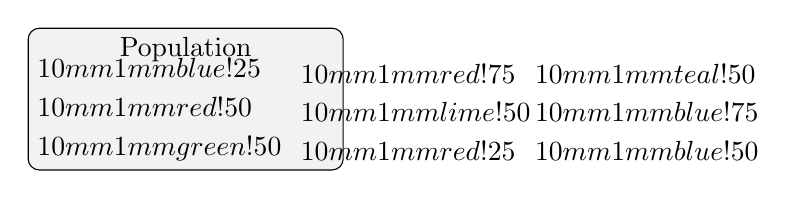
\begin{tikzpicture}
  \tikzstyle{box} = [rectangle, rounded corners, minimum width=4cm, minimum height=1.8cm,text centered, draw=black, fill=gray!10]

  % Population
  \node [box] (population) {};
  \node [anchor=north] at (population.north) {Population};

  \node (line1) [anchor=south west] at (population.south west) {$\coloredrule{10mm}{1mm}{green!50}$};
  \node (line2) [anchor=south west] at (line1.south east) {$\coloredrule{10mm}{1mm}{red!25}$};
  \node (line3) [anchor=south west] at (line2.south east) {$\coloredrule{10mm}{1mm}{blue!50}$};
  \node (line4) [anchor=south west] at (line1.north west) {$\coloredrule{10mm}{1mm}{red!50}$};
  \node (line5) [anchor=south west] at (line2.north west) {$\coloredrule{10mm}{1mm}{lime!50}$};
  \node (line6) [anchor=south west] at (line3.north west) {$\coloredrule{10mm}{1mm}{blue!75}$};
  \node (line7) [anchor=south west] at (line4.north west) {$\coloredrule{10mm}{1mm}{blue!25}$};
  \node (line8) [anchor=south west] at (line5.north west) {$\coloredrule{10mm}{1mm}{red!75}$};
  \node (line9) [anchor=south west] at (line6.north west) {$\coloredrule{10mm}{1mm}{teal!50}$};

\end{tikzpicture}